\documentclass{amsbook}

\usepackage[a5paper,margin=28mm,marginparwidth=20mm,marginparsep=3mm]{geometry}
\usepackage{verse,microtype,mathtools,xfrac,marginnote,graphicx,ragged2e,xstring,afterpage,pifont}

\usepackage{fontspec}
\usepackage[T1]{fontenc}
\newfontfamily\hoskeroe{English Towne}
\newfontfamily\greekish{CMU Serif}
\newfontfamily\arabicish{KacstQurn}
\newfontfamily\frakturish{Fette UNZ Fraktur}
\setmainfont[Numbers=OldStyle]{Latin Modern Roman}
\newfontfamily\scshape[Letters=SmallCaps]{Latin Modern Roman Caps}

\usepackage[hidelinks]{hyperref}

\newcommand{\addpoemtolist}[1]{}
\newcommand{\poeticmarginnote}[1]{\marginnote{\footnotesize #1}}

\newcounter{pageoffset}
\newcounter{pagedifference}

\newcommand{\poemone}{}
\newcommand{\poemtwo}{}
\newcommand{\poemthree}{}
\newcommand{\printpoems}{%
  \setcounter{pagedifference}{\value{page}-\value{pageoffset}}
  \IfEq{\thepagedifference}{2}
  { \poemone \clearpage}{}
  \IfEq{\thepagedifference}{5}
  {\poemtwo \clearpage
   \poemthree \clearpage}{}
  \afterpage{\printpoems}%
}
\newcommand{\initprintpoems}{
  \setcounter{pageoffset}{\thepage-1}
  \afterpage{
  \printpoems
  }
}
\newcommand\blfootnote[1]{%
  \begingroup
  \renewcommand\thefootnote{}\footnote{#1}%
  \addtocounter{footnote}{-1}%
  \endgroup
}

\title{The First Book. Lucifer in Starlight}

\begin{document}
\frontmatter
\renewcommand\thefootnote{{}}
\maketitle

\thispagestyle{empty}
\topskip0pt
\vspace*{\fill}
\noindent {\it How you are fallen from heaven, Lucifer, son of the morning. How you are cut down to the ground, you who laid nations low. You said in your heart, I will ascend into heaven; I will exalt my throne above the stars of God; I will ascend above the heights of the clouds; I will make myself like the Most High. But you are brought down to hell, to the depths of the pit...}
\vspace*{\fill}
\clearpage

\tableofcontents

\thispagestyle{empty}
\topskip0pt
\vspace*{\fill}
{\centering
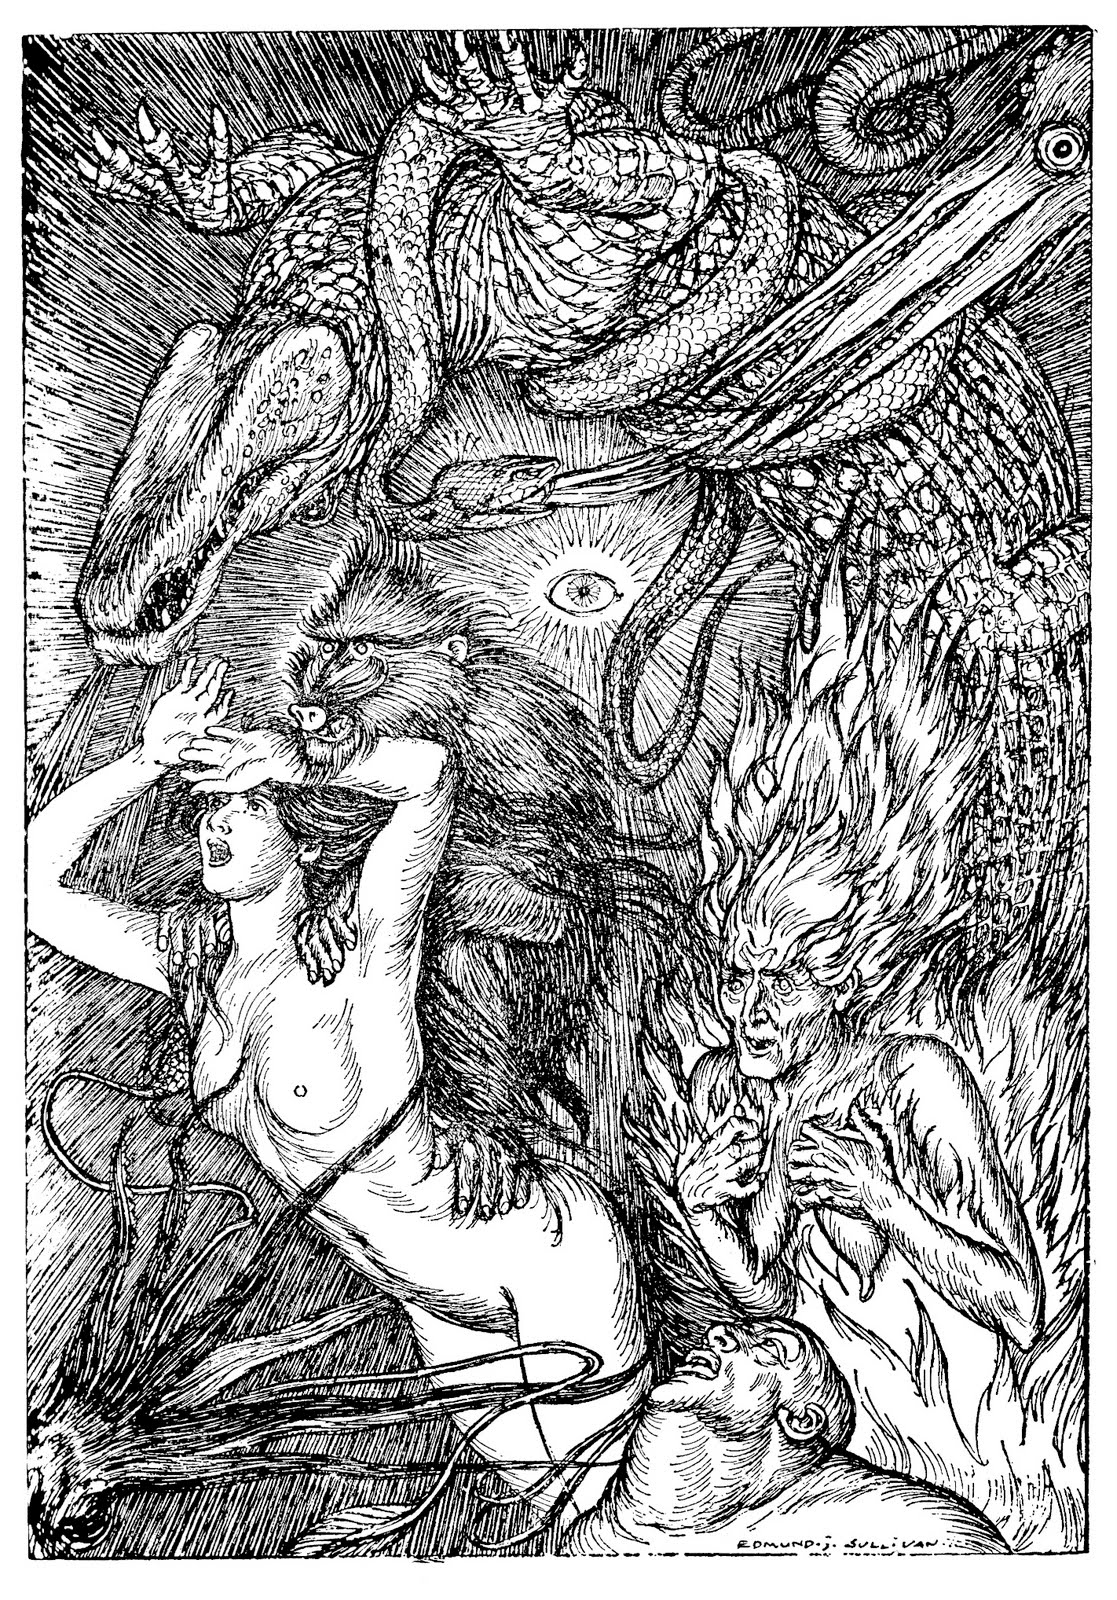
\includegraphics[width=\textwidth]{images/placeholder_image.jpg}}
\vspace*{\fill}
\clearpage

\thispagestyle{empty}
\topskip0pt
\vspace*{\fill}
\noindent {\sc Argument:} {\itshape How the two lovers from \emph{William's Farewell}, having suffered an unrecoverable loss, wandered across the country; and of the strange things that befell them on their way.}
\vspace*{\fill}
\clearpage

\thispagestyle{empty}
\topskip0pt
\vspace*{\fill}
{\centering
\includegraphics[width=\textwidth]{#AUTUMNAL_IMAGE}}
\vspace*{\fill}
\clearpage

\mainmatter

\chapter{Autumnal}

\renewcommand{\poemone}{
\begin{figure*}[p!]
\bigskip
\ding{72}
\bigskip
#AUTUMNAL_POEM_1
\end{figure*}
}
\renewcommand{\poemtwo}{
\begin{figure*}[p!]
\bigskip
\ding{72}
\bigskip
#AUTUMNAL_POEM_2
\end{figure*}
}
\renewcommand{\poemthree}{
\begin{figure*}[p!]
\bigskip
\ding{72}
\bigskip
#AUTUMNAL_POEM_3
\end{figure*}
}
\initprintpoems

#AUTUMNAL_PROSE
\clearpage

\thispagestyle{empty}
\topskip0pt
\vspace*{\fill}
{\centering
\includegraphics[width=\textwidth]{#HIBERNAL_IMAGE}}
\vspace*{\fill}
\clearpage

\chapter{Hibernal}

\renewcommand{\poemone}{
\begin{figure*}[p!]
\bigskip
\ding{72}
\bigskip
#HIBERNAL_POEM_1
\end{figure*}
}
\renewcommand{\poemtwo}{
\begin{figure*}[p!]
\bigskip
\ding{72}
\bigskip
#HIBERNAL_POEM_2
\end{figure*}
}
\renewcommand{\poemthree}{
\begin{figure*}[p!]
\bigskip
\ding{72}
\bigskip
#HIBERNAL_POEM_3
\end{figure*}
}
\initprintpoems

#HIBERNAL_PROSE
\clearpage

\thispagestyle{empty}
\topskip0pt
\vspace*{\fill}
{\centering
\includegraphics[width=\textwidth]{#VERNAL_IMAGE}}
\vspace*{\fill}
\clearpage

\chapter{Vernal}

\renewcommand{\poemone}{
\begin{figure*}[p!]
\bigskip
\ding{72}
\bigskip
#VERNAL_POEM_1
\end{figure*}
}
\renewcommand{\poemtwo}{
\begin{figure*}[p!]
\bigskip
\ding{72}
\bigskip
#VERNAL_POEM_2
\end{figure*}
}
\renewcommand{\poemthree}{
\begin{figure*}[p!]
\bigskip
\ding{72}
\bigskip
#VERNAL_POEM_3
\end{figure*}
}
\initprintpoems

#VERNAL_PROSE
\clearpage

\thispagestyle{empty}
\topskip0pt
\vspace*{\fill}
{\centering
\includegraphics[width=\textwidth]{#AESTIVAL_IMAGE}}
\vspace*{\fill}
\clearpage

\chapter{Aestival}

\renewcommand{\poemone}{
\begin{figure*}[p!]
\bigskip
\ding{72}
\bigskip
#AESTIVAL_POEM_1
\end{figure*}
}
\renewcommand{\poemtwo}{
\begin{figure*}[p!]
\bigskip
\ding{72}
\bigskip
#AESTIVAL_POEM_2
\end{figure*}
}
\renewcommand{\poemthree}{
\begin{figure*}[p!]
\bigskip
\ding{72}
\bigskip
#AESTIVAL_POEM_3
\end{figure*}
}
\initprintpoems

#AESTIVAL_PROSE

\bigskip
\bigskip
\begin{center}
{\sc End of the First Book}
\end{center}

\end{document}
